\chapter{DevOps}
In the old-style software engineering there are \textbf{separate} teams addressing software development, deployment, release and support.
The development team, or a separate maintenance team, is responsible for software updates and maintenance.\\
This approach introduces many issues, which can be summarized as \textbf{difficult communication} amongst teams, due to different tools, skills, etc. leading to requiring multiple to days to release an "urgent" patch.

\textit{Amazon} re-engineered its software into (micro)services assigning both service development and service support to the same team.

\section{Principles}

\labelitemize{\textbf{\textit{\underline{Principles}}}
}{
   \begin{enumerate}[label=\textbf{D\arabic*} - ,left=1em]
      \item \textit{Everyone is responsible for
      everything.}
      \begin{enumerate}
         \item 
         All team members have joint responsibility
         for developing, delivering, and supporting the
         software.
      \end{enumerate}
      \item \textit{Everything that can be automated
      should be automated}
      \begin{enumerate}
         \item 
         All activities involved in testing, deployment,
         and support should be automated if it is possible
         to do so. There should be mimimal manual
         involvement in deploying software.
      \end{enumerate}
      \item \textit{Measure first, change later}.
      \begin{enumerate}
         \item 
         DevOps should be driven by a measurement
         program where you collect data about the
         system and its operation. You then use the
         collected data to inform decisions about
         changing DevOps processes and tools.
      \end{enumerate}
   \end{enumerate}
}
\nl
\nl

\labelitemize{\textit{Benefits}}{
\begin{enumerate}
   \item \textit{Faster deployment}\\
   Software can be deployed to production more
   quickly because communication delays between
   the people involved in the process are dramatically
   reduced.
   \item \textit{Reduced risk}\\
   The increment of functionality in each release is
   small so there is less chance of feature interactions
   and other changes that cause system failures and
   outages.
   \item \textit{Faster repair}\\
   DevOps teams work together to get the software
   up and running again as soon as possible. There is
   no need to discover which team was responsible for
   the problem and to wait for them to fix it.
   \item \textit{More productive teams}\\
   DevOps teams are happier and more productive
   than the teams involved in the separate activities.
   Because team members are happier, they are less
   likely to leave to find jobs elsewhere.
\end{enumerate}
}

\section{Code Management}

\begin{figure}[htbp]
   \centering
   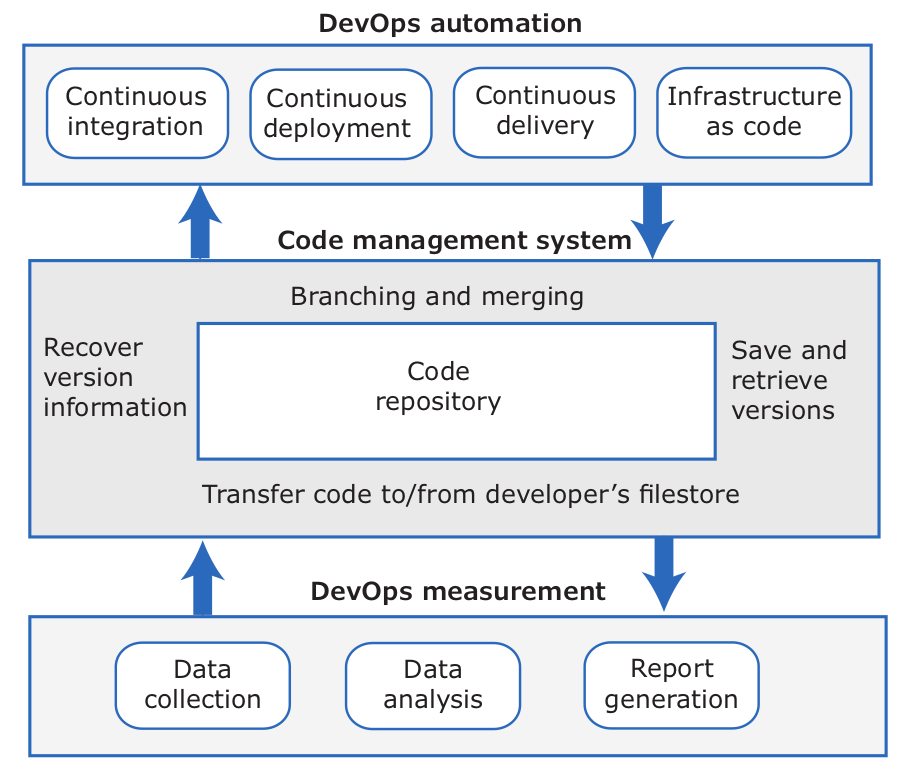
\includegraphics{images/codemanagement.png}
   \caption{Code management according to DevOps}
   \label{fig:codemanagement}
\end{figure}

Code must be \textbf{managed} using \texttt{git}, which is a \textit{decentralized system} which provides some crucial benefits:
\begin{enumerate}
   \item \textbf{Resilience}
   \begin{enumerate}
      \item Every dev has its \textit{own copy} of the project
      \item If the shared repository is damaged or subjected to a cyber-attack, work can continue and a previous state may be \textit{restored}
      \item Devs can \textit{work offline}
   \end{enumerate}
   \item \textbf{Speed}
   \begin{enumerate}
      \item Committing changes to the repository is a fast, \textit{local} operation
   \end{enumerate}
   \item \textbf{Flexibility}
   \begin{enumerate}
      \item Local experimentation is much simpler i.e. 
      Developers can safely try different approaches without exposing their experiments to other project members
   \end{enumerate}
\end{enumerate}

\section{Automation}

\texttt{GitHub} provides a mechanism called \textbf{WebHooks} which trigger DevOps \textbf{automation tools} in respose to updates to the project repository.

\subsection{Continuous integration}
\textbf{Continuous integration} means that every time that a dev commits a change to project's main branch, 
an \textit{updated executable} version of the system is \textbf{built} and \textbf{tested}.

System \textbf{integration} ($\rightarrow building$) is more than simply "compiling source code", but includes many steps like installing \texttt{db} software, loading test data, preparing config files, running system tests, and so on.\\
If a system is \textit{infrequently integrated}, problems can be difficult to isolate, and fixing them would considerably slow down system development.

With continuous integration, an integrated version of the system is created and tested \underline{every time a change is pushed} to the system’s shared code repository.
On completion of the push operation, repository sends message
to integration server to build a new version of the product.

\subsubsection{Breaking the Build}

To avoid breaking a working build, usually an \textbf{"integrate twice"} approach is preferred:
the integrated system version is created and tested \textbf{locally}, and then {---}if tests succeed{---} the changes get pushed to the project repository and the main integration server gets triggered,
resulting in a new official build. 

Besides, no dev wants the stigma of "breaking the build", so everyone is very careful and check its code before pushing to project repo.


\subsection{Continuous delivery and Deployment}
\textbf{Continuous delivery} {--}and \textit{deployment}{--} refers to the testing environment, which must be the product's operating environment.
\note{
   \textbf{Continuous deployment} means that every new release of the system should be seamlessy made available to users as soon as a change gets committed\footnote{Shouldn'it be tested first? \smiley} to the main branch.
}
With continuous \textit{integration}, new system builds get tested {--}locally by devs and{--} by the integration server, but such development differs from the \textbf{real production environment}.
The production server may have different filesystem organization, access
permissions, installed applications;
in other words, new bugs may show up.

Continuous delivery ensures that changed system is ready for \textbf\underline{{delivery}
to customers},
by performing 
\textbf{feature tests} in \textit{production} environment
 to make sure that environment does not cause system failures, and
\textbf{load tests} to check how software behaves as number of users increases.
\note{
   Containers are the simplest way to create a replica of a production
environment.
   }

So, in order to \textbf{deliver}, after initial integration testing a staged test environment must be configured to crete a \textbf{replica} of production environment,
where \textbf{acceptance tests} on \textit{functionality}, \textit{load} and \textit{performance} can be ran into.

Continuous \textbf{deployment} is practical only for cloud-based systems and can be instead can be summarized in three steps:
\begin{enumerate}
   \item software and data are transferred to
   production servers
   \item new service requests stopped, older
   version processes outstanding
   transactions
   \item switch to new system version and
   restart processing
\end{enumerate}

However note that, there may be \textbf{business reasons} to \textit{\underline{avoid} deploying} every system change to customers,
like the presence of incomplete features, too frequent UI changes, or desire/need to synchronize releases with known business cycles\footnote{solar/academic year, seasons, tax payments...}

\subsection{Infrastructure as Code}
Manually maintaining a computing infrastructure with tens or
hundreds of servers is expensive and error-prone:
different servers may require different dependencies, drivers, packages... some may be virtual, others physical...

The process of updating software on servers should be automated by using a \textbf{machine-readable model} of the infrastructure $\longrightarrow$ \textit{"Infrastructure as Code"}.

\textit{Configuration Management} (\texttt{CM}) tools, like
\textit{Puppet} and \textit{Chef and Ansible}, can
automatically install software and services
on servers according to the infrastructure
definition, so that when changes have to be made,
the infrastructure model is updated and CM tool makes the changes to all servers.

This provides tracking and prevents all the human-based errors related to configuring, installing and managing software on servers, 
ultimately resulting in many advantages:
\begin{enumerate}
   \item \textbf{Visibility}\\
   Infrastructure defined as stand-alone model that can be
   read/understood/reviewed by whole DevOps team.
   \item \textbf{Reproducibility}\\
   Installation tasks will always be performed in the same sequence, same
   environment will be always created. You do not have to rely on people
   remembering the order that they need to do things.
   \item \textbf{Reliability}\\
   Automation avoids simple mistakes made by system administrators when
   making same changes to several servers.
   \item \textbf{Recovery}\\
   Infrastructure model can be versioned and stored in a code management
   system. If infrastructure changes cause problems, you can easily revert
   to older version and reinstall the environment that you know works.
\end{enumerate}
\nl

Summing up, \textbf{Infrastructure as Code} indicates that instead of delegating the system infrastructure managing to human administrators or developers,
\textit{machine-readable} models of the infrastructure \footnote{network, servers, routers, etc.} should be provided, on which the product executes
are used by configuration management tools to automatically build the
software’s execution platform; 
the software to be installed, such as compilers, libraries, DBMS, packages and so on, is included in the infastructure model.


\section{Measuring DevOps}
Your own DevOps process should be continuously measured in order to improve it and thus to enhance software quality and reduce deployment times.

\begin{enumerate}
   \item \textbf{Process} measurements\\
   collect and analyze data on development/testing/deployment processes
   \item \textbf{Service} measurements\\
   collect and analyze data on software’s performance/reliability/acceptability to customers
   \item \textbf{Usage} measurements\\
   collect and analyze data on how customers use your product
   (help you identify issues and problems with the software itself)
   \item \textbf{Business success} measurements\\
   collect and analyze data on how your product contributes to overall business success
   \note{
      hard to isolate contribution of DevOps to business success - that may be due e.g. to
      DevOps introduction or to better managers
   }
\end{enumerate}

Measuring software and its development, should be automated but is a complex process:
defining suitable metrics and ways to collect them is away from trivial.
\note{
   Consider the basic example of record \textit{lead time} for implementing a change: 
   is the \textit{"lead time"} the overall elapsed time or the time spent by developers? How to take into account higher priority changes whose implementation slowed down other changes?
}

\begin{figure}[htbp]
   \centering
   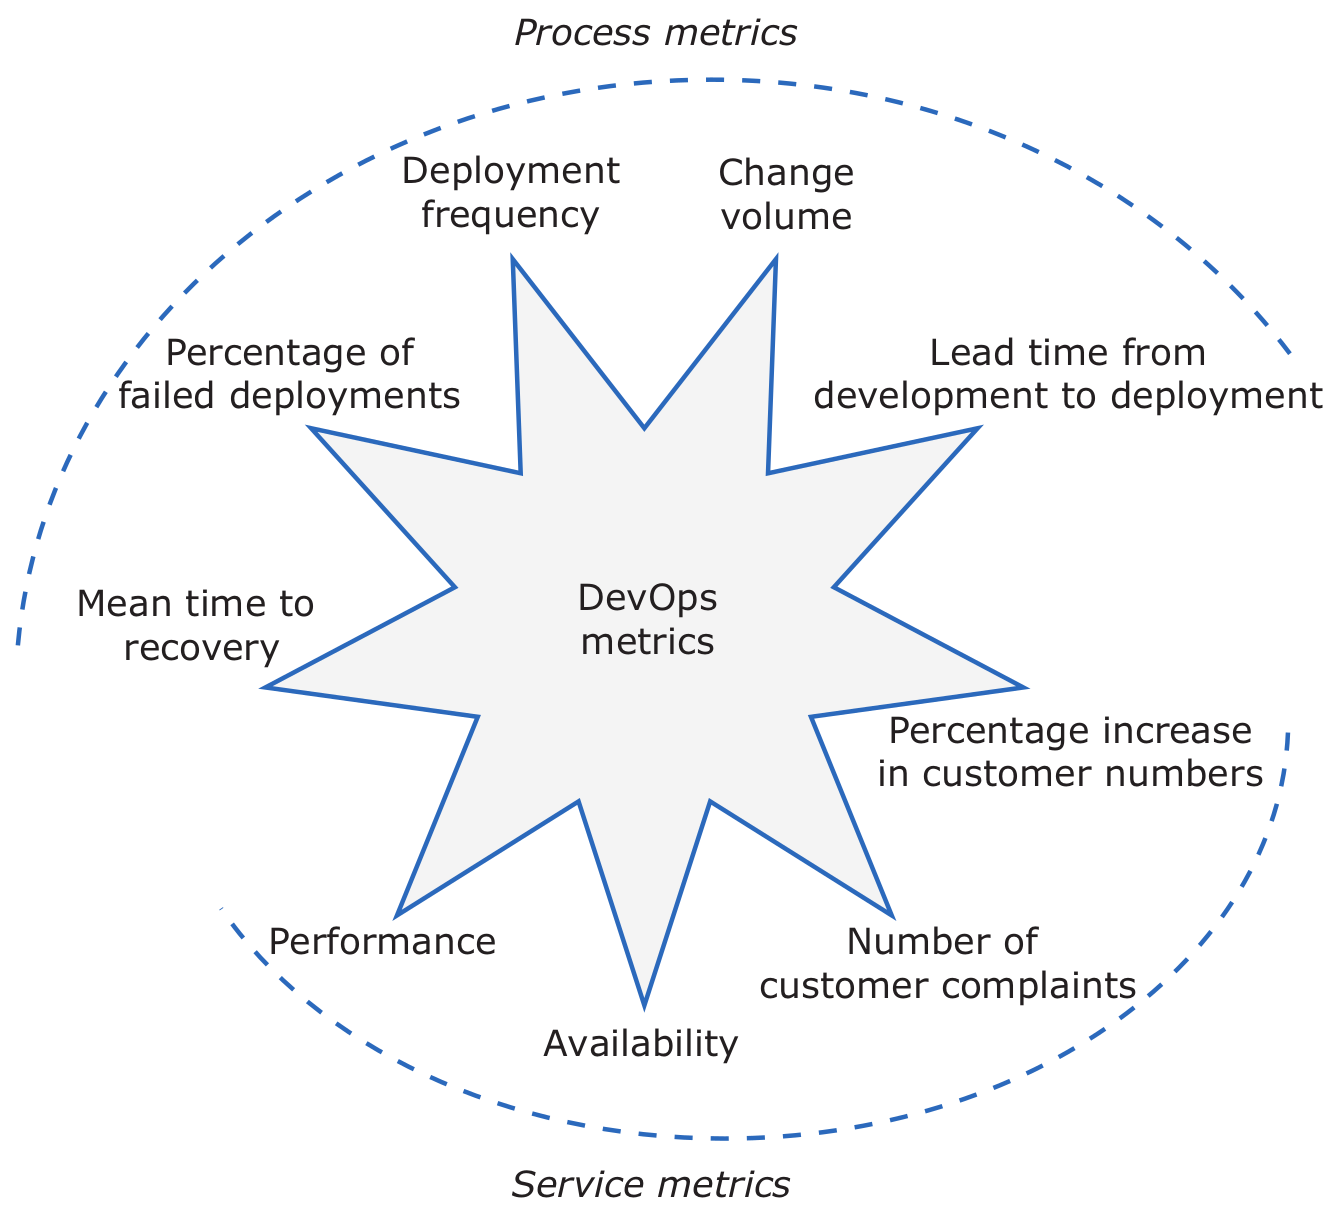
\includegraphics{images/devops_metrics.png}
   \caption{DevOps Metrics}
   \label{fig:devops_metrics}
\end{figure}

\labelitemize{\textit{\underline{Collecting data}}}{
\begin{enumerate}
   \item Use \textbf{continuous integration tools} like \textit{Jenkins} to collect data on \textit{deployments}, successful tests, etc.
   \item Use \textbf{monitoring services} featured by cloud providers like \textit{Amazon’s Cloudwatch} to collect data on \textit{availability} and \textit{performance}
   \item Collect \textit{customer-supplied data} from \textbf{issue management systems}
   \item Add \textbf{instrumentation} to your product to gather data on its
   performance and how it is used by customers
   \begin{enumerate}
      \item use \texttt{log} files, where \texttt{log} entries are timestamped events reflecting customer actions and/or
      software responses
      \item \texttt{log} as many events as possible
      \item use available \texttt{log} analysis tools to extract useful information about on how your software is
      used
   \end{enumerate}
\end{enumerate}
}